\Subsection{Арифметические действия с пределами функций}

a - предельная точка $ E \subset R $ \\
$ f, g : E \rightarrow R $ \\
$ \lim\limits_{x \rightarrow a} f(x) = A \in \overline{\R} $\\
$ \lim\limits_{x \rightarrow a} g(x) = B \in \overline{\R} $\\
Если операции определены на $ \overline{\R}$:
\begin{enumerate}
	\item $ \lim\limits_{x \rightarrow a} (f(x) \pm g(x)) = A \pm B $
	\item $  \lim\limits_{x \rightarrow a} (f(x) \cdot g(x)) = A \cdot B $
	\item $  \lim\limits_{x \rightarrow a} (\dfrac{f(x)}{g(x)}) = \dfrac{A}{B} $ 
	\item $  \lim\limits_{x \rightarrow a} (|f(x)|) = |A| $
\end{enumerate}
\begin{proof}
	$ \forall (x_n) - $ последов, $ x_n \in E \setminus \{a\} , x_n \rightarrow a $ \\
	$ f(x_n) \rightarrow A, g(x_n) \rightarrow B,  f(x_n) \pm g(x_n) \rightarrow A \pm B $\\
	$ \Rightarrow \lim\limits_{x \rightarrow a} (f(x) \pm g(x)) = A \pm B $
\end{proof}
$ f(x) \rightarrow \infty \Leftrightarrow |f(x)| \rightarrow +\infty $\\

\Section{Непрерывные функции}

\begin{definition}
	$ f : E \rightarrow, E \subset \R$\\
	$ f $ непрерывна в a, если \\
	1. a - не предельная точка \\
	2. а - предельная точка и предел функции в этой точке равен её значению 
	
	$ f : E \rightarrow \R $ \\
	1. f непр в а \\
	2. $ \forall \eps > 0 \exists \delta > 0 : x\in E, | x - a | < \delta \rightarrow |f(x) - f(a) | \leq \eps $\\
	3. Прообраз любой окрестности $ f(a) - $ окрестность а в $E$ \\
	Т.е. $ U \cap E, $ где $ U \subset \R $ т.ч. $ \exists \eps > 0 \  (a-\eps, a+\eps) \subset U$\\
	4. Для любой посл. $ x_n $ т.ч. $ x_n \in E $ и $ x_n \rightarrow a $ вып $ f(x_n) \rightarrow f(a) $
	
	\begin{proof}
	Пусть а не предельная точка \\
	1. По определению \\
	2. Выполняется при достаточно маленьких $ \delta  > 0$ $ |x-a| < \delta, x \in E \Rightarrow x = a $ \\
	3. $U'$ - окрестность  $ f(a) $в$ \R$ \\
	$ \Rightarrow f(a) \in U' \Rightarrow a \in f^{-1}( U' ) $ \\
	$ \{a\} = U_{\delta} (a) \cap E $ при нек $ \delta > 0 $ $\Rightarrow \{a\} - $ окр-ть а в Е \\
	$ \Rightarrow  f^{-1}(U') = $\\
	4. $ x_n \rightarrow a, x_n \in E \Rightarrow \exists N, \forall n \geq N : x_n = a \Rightarrow f(x_n) \rightarrow f(a) $ \\ %pic1@
	Пусть а - предельная точка \\
	 $ 1 \Rightarrow 2 $ 
	 $ \forall \eps > 0, \exists \delta > 0, x\in \dot{U}_{\delta} (a) \Rightarrow f(x) \in U_{\eps} (f(a)) $ \\
	 Кроме того $ f(a) \in U_{\eps}(f(a)) \Rightarrow \forall \eps > 0, \exists \delta > 0 : x \in U_{\delta} (a) \Rightarrow f(x) \in U_{\eps} (f(a)) $
	 $ 2 \Rightarrow 1 $ т.е. $ \lim\limits_{x \rightarrow a} f(x) = f(a) $\\
	 $ 1 \Rightarrow 3  \ \  U(f(a)) \supset U_{\eps} (f(a)) (\eps > 0) \supset f(U_{\delta}(a)) $ (при нек $delta > 0$ ) \\ % pic2@
	 $ U_{\delta}(a) \subset f^{-1} (U(f(a))) \Rightarrow f^{-1} (U(f(a))) \supset U_{\delta} (a) \cap E \Rightarrow $ окр-ть а в E \\
	 $ 3 \Rightarrow 2 \ \ \eps > 0, f'(U_{\eps} (f(a))) \supset U_E(a) =U_{\R}  \cap E \supset U_{\delta} (a) \cap E, \delta > 0 $ \\
	 Тогда $ x \in U_{\delta} (a) \cap E \Rightarrow f(x) \in U_{\eps} (f(a)) $ \\
	 
	 $ 1 \Rightarrow 4 \lim\limits_{x \rightarrow a} f(x) = f(a) $ \\
	 1. В $ (x_n) $ лишь конечное число членов, равных а \\
	 Тогда можно их выкинуть и это не повлияет на предел. \\
	 $ x_{n_k} -$  подпосл членов, отличных от а \\
	 $ f(x_{n_k}) \rightarrow f(a) ]\Rightarrow f(x_n) \rightarrow f(a)$ \\
	 2. В $	(x_n) $ лишь конечное число членов, отличных от а \\
	 $ (x_{n_k}) - $ подпослед из всех членов, равных а \\
	 $ f(x_{n_k}) = f(a) \rightarrow f(a) $\\
	 3. Бесконечно много $ = a$ и $ \neq a $ \\
	 $ (x_{n_k}) $ из всех, равных а \\
	 $ (x_{n'_k}) $ из всех, не равных а \\
	  $ f(x_{n_k}) = f(a) \rightarrow a $\\
	   $ f(x_{n'_k}) = f(a) \rightarrow a \Rightarrow f(x_n) \rightarrow a$\\
	 $ 4 \Rightarrow 1  $ Пусть $(x_n) $ - посл-ть \\
	 $ x_n \rightarrow a, x_n \neq a, \forall n $ \\
	 Из опр по Гейне $ \lim\limits_{x \rightarrow a} f(x) = f(a) $
	  \end{proof}
	 
\end{definition}
Замечание\\
Пусть $ a \in E $ Тогда окр-ть $a$ в $ E $ - мн-ва, содержащие $ U_{\delta} (a) \cap E $ для к-л $ \delta > 0 $ \\
%pic3

\Subsection{Свойства непрерывных ф-ций}

\begin{properties}
	Пусть $ f, g : E \rightarrow \R, a \in E$ \\
	 $ f, g $ - непрерывны в а. Тогда \\
	 \begin{enumerate}
	 	\item $ f \pm g $ непр. в а
	 	\item $ fg $ непр. в a 
	 	\item Если  $ g(a) \neq 0, \dfrac{f}{g} $ непр.
	 	\item $|f|$ непр. в $a$
	 \end{enumerate}
% 	\begin{proof}
 		% pic4
% 	\end{proof}
 	Многочлены непрерывны 
	\begin{consequence}
		Пусть $ g_1, \ h \in \R[x] $ \\
		$ E = \{ x | h(x) \neq 0 \} $ \\
		$ f : E \rightarrow \R $ \\
		$ x \mapsto \dfrac{g(x)}{h(x)} $ \\
		Тогда f непрерывна во всех точках Е \\
		
 	\end{consequence}
 \begin{predl}
 	 $ f : E_1 \rightarrow \R , g : E_2 \rightarrow \R$ \\
 	$ f(E_1) \subset E_2 $ \\
 	f непр в a  $ \in E_1 $ g непр  в $ f(a)$\\
 	Тогда $ g \circ f $ непр в $ a $ 
 	\begin{proof}
 		$ x_n \rightarrow a, x_n \in E_1 $ \\
 		$ \Rightarrow f(x_n) \rightarrow f(a), f(x_n) \in E_2 $\\
 		$ \Rightarrow g(f(x_n))  \rightarrow g(f(a))$ \\
 		$ (g\circ f) (x_n) $\\
 		$ g \circ f $ непр. в а 	
 	\end{proof}
 \end{predl}
  \begin{theorem}
  	Теорема о стабилизации знака \\
  	Пусть $ f : E \rightarrow \R  $ непр. в тчк. а, $ f(a) > 0$\\
  	Тогда $ f(x) > 0 $ в нек окрестности $a$ \\
  	$ f(a) \in (0, +\infty) $ \\
  	$ f^{-1} ((0, +\infty)) $ окр-ть в Е
  \end{theorem}
\end{properties} 

\begin{lemma}
	Пусть $ 0 < x < \dfrac{\pi}{2} $ Тогда $ \sin x < x < \tan x $\\
	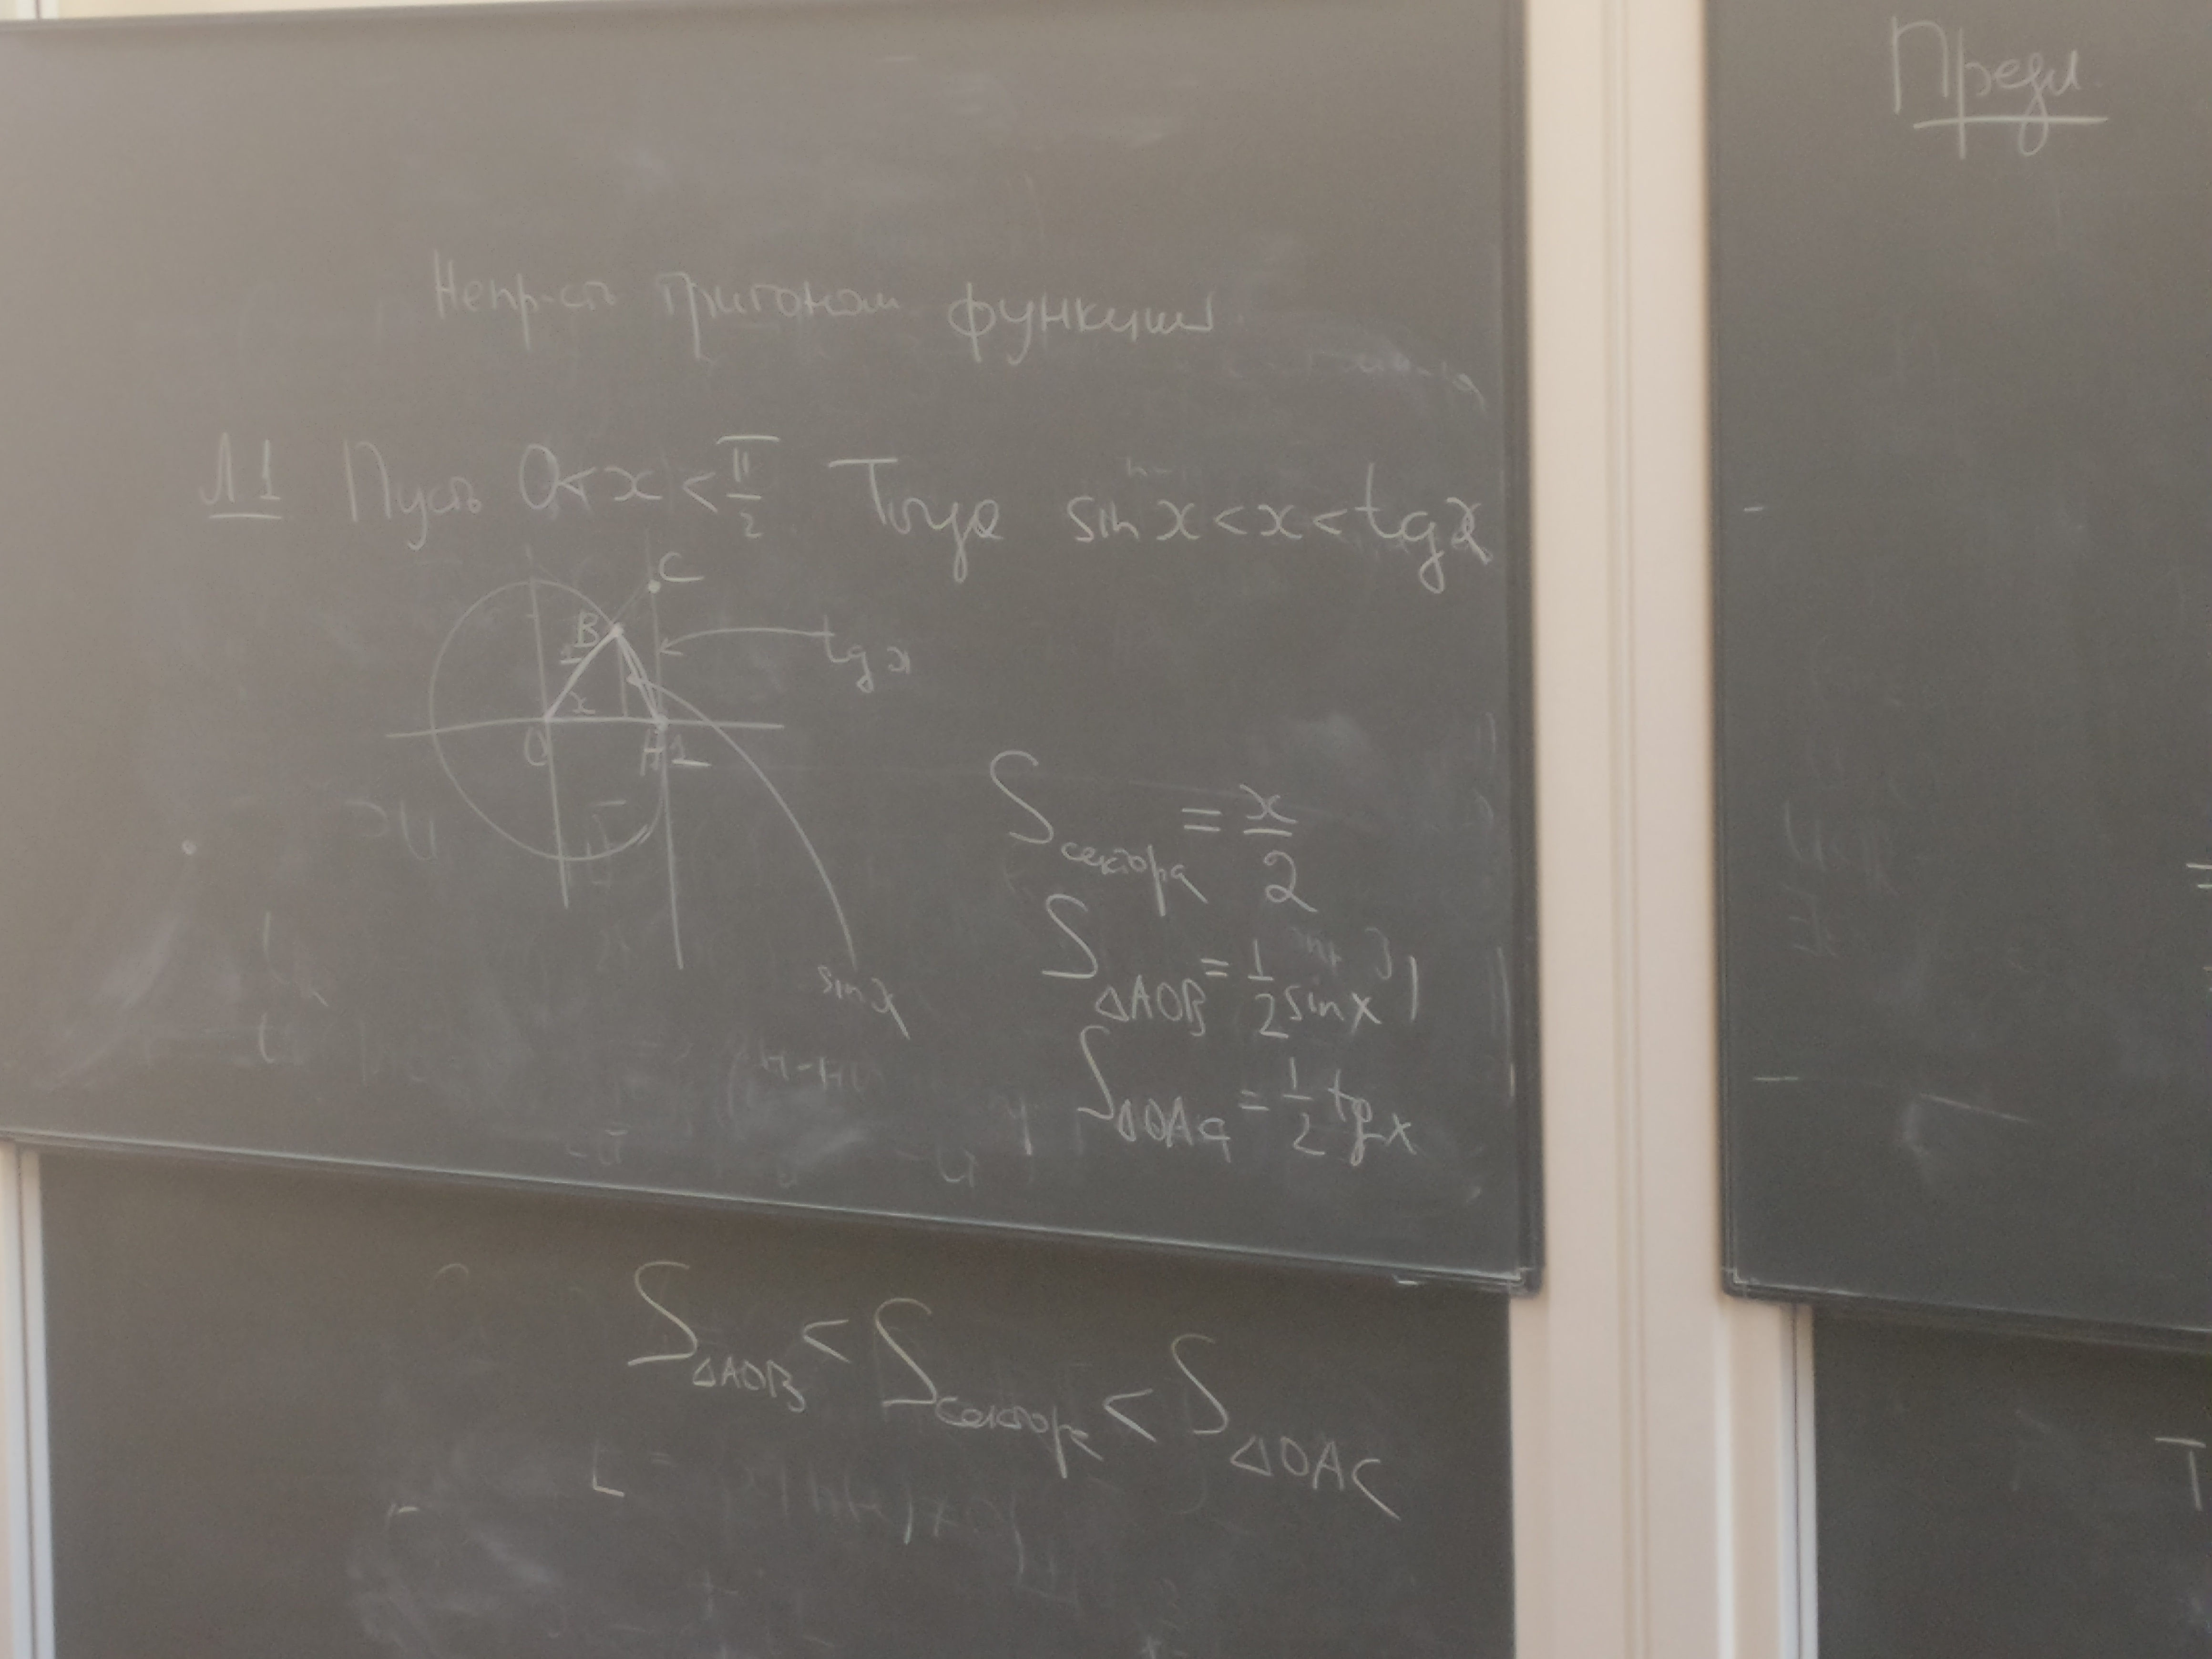
\includegraphics[width=0.9\linewidth]{IMG_20181015_142326}
\end{lemma}
\begin{consequence}
	\begin{enumerate}
	 \item 	$ |\sin(x) | \leq |x| \forall x \in \R , |\sin(x)| = | x| $ только при $x = 0$ \\
	 $ |x| < \dfrac{\pi}{2} \Rightarrow | \sin(x) | < |x| $ по лм. 1 \\
	 $ |x| > \dfrac{\pi}{2} \Rightarrow |x| > 1 > |sin(x)| $ 
	 \item $ |\sin x - \sin y | \leq | x - \overline{y} | $\\
	 \item $ \sin x, \cos x $ - непрерывные ф-ции\\
	 $ \sin^{-1} (U_{\eps} f(x)) \supset U_{\eps } (x) $\\
	 $ |y - x| < \eps \Rightarrow |\sin y - \sin x| < \eps $ \\
	 $ \cos x = \sin (x + pi / 2) $ непрерывна как композиция 
	 \item $ \tan x, \cot x $ непрерывны на своей области определения
	 
	\end{enumerate}

\end{consequence}

\begin{theorem}
	Теорема Вейерштрасса\\
	Пусть f непрерывна на $[a, b] $. Тогда f достигает наибольшего и наименьшего значения на $ [a,b]$ 
	\begin{proof}
		1. Докажем, что  f ограниченная на $[a, b] $ \\
		Предположим, что f не ограничеа сверху\\
		Это будет означать, что $ \forall n \in \N \exists x_n \in [a, b]  : f(x_n) > n $ \\
		$x_n$ - ограниченная послед, значит содержит сходящуюся подпоследовательность $ (x_{n_k})  \rightarrow c \in [a, b] $ \\
		В силу непрерывности $ f(x_{n_k}) \rightarrow f(c) $\\
		$ f(x_n) \rightarrow +\infty \Rightarrow f(x_{n_k}) \rightarrow +\infty $\\
		Противоречие. Аналогично f огр. снизу
		2. $ M = \sup \{ f(x) | x \in [a, b]  \} \in \R $ \\
		Предположим, что M не достигается $ \forall x, \in [a, b] , f(x) \neq M $ \\
		$ g : [a, b] \rightarrow \R $ \\
		$ x \mapsto \dfrac{ 1}{M - f(x)} $ \\
		G непрерывна как отношение непрерывных ф-ций.\\
		$ \exists c > 0, \forall x \in [a, b]  : g(x) < C, \dfrac{1}{M - f(x)} < C \Leftrightarrow M - f(x) > \dfrac{ 1}{C} \Leftrightarrow f(x) < M - \dfrac{ 1}{C}  < M \Rightarrow M - \dfrac{1}{C}$ верхняя граница H - противоречие \\
		Т. е. $ \exists x \in [a, b] : f(x) = M $ 
	\end{proof}
\end{theorem}
\begin{consequence}
	$ [a, b] = [b,a] $ если $ a > b $
	\begin{enumerate}
		\item (Принцип Больцано-Коши) f непрерывн. на $[a, b] $, y - число на $ [f(a), f(b)] $ Тогда $ \exists c \in [a, b]  : f(c) = y$ %pic6
		\begin{proof}
			Пусть для опред. $ f(a) \leq f(b) $\\
			$ M = \{ x \in [a, b] | f(x) \leq y \} $\\
			Пусть $ x_0 = \sup M$ 
			$ [x, x_0] \supset M $ Пусть $y_0 $ - наиб значение f на этом отрезке. Если $ y_0 = y $ - доказано \\
			Иначе $ y_0 < y $ \\
			$ \forall n \in \N $ пусть $ x_n \in M $ таково, что $x_n> x_0 - \dfrac{1}{n} $  \\
			$ x_n \rightarrow x_0 $ \\
			$ f(x_n) \rightarrow f(x_0), f(x_n) \leq y_0 $\\
			$ \Rightarrow f(x_0) \leq y_0 $%pic7@
			$ \exists \delta > 0  \ \ f(x) in (-\infty, y) $ при $x \in U_{\delta} (x_0) \Rightarrow U_\delta (x_0) \subset M \subset [a, x_0] $ 			
		\end{proof}
		\item $ f: [a, b]  \rightarrow \R $ f - непрерывна \\
		Тогда $ f([a, b] ) $ - отрезок \\
		\begin{proof}
			$ m = \min f(x), x \in [a, b] $ \\
			$ M = \max f(x), x \in [a, b]  $  \\
			$f(x) < M - \dfrac{1}{C} < M $ \\
			$ f( [a, b] ) \subset{[m, M]} $ \\
			$ \exists c, f(c) = m, \exists d, f(d) = M $ \\
			$ m \leq y \leq M \Rightarrow \exists x \in [c,d] : f(x) = y $ \\
			Т.е. $ f([a, b] ) = [m, M] $ \\ 
		\end{proof}
		Промежутки - $ [a,b], [a, b), (a, b], (a, b) $ - конечные промежутки\\
		$ (a, + \infty), (-\infty, a), [a, + \infty), (-\infty, a], \R $ - бесконечные промежутки \\
		\item Пусть I - промежуток,  f непрерывн. на I \\
		Тогда $ f(I) - $ промежуток
		\begin{proof}
			I - нек промежуток \\
			$ m = \inf f(I) \in \overline{\R} $ \\
			$ M = \sup f(I)  \in \overline{\R} $ \\
			$ (m, M) \subset f(I) $ \\
			$ y \in (m, M) , \exists y_0 \in I, y_0 < y $ т.к. $ y \neq m $ \\
			$ y_0 = f(x_0), x_0 \in I $ \\
			$ \exists y_1 \in f(I), y_1 > y (y_1 \neq M)$ \\
			$ y_1 = f(x_1), x_1 \in I$\\
			$ \exists x \in [x_0, x_n] : f(x) = y,$ т.е. $ y \in f(I) $ \\
			$ (m, M) \subset I $\\
			$ m = \inf I, M = \sup I $
			$ f(I) = [m,M], [m, M), (m, M], (m, M) $
		\end{proof}
	\end{enumerate}
\end{consequence}

\Subsection{Обратная функция}
\noindent
$ f : X \rightarrow Y $ - биекция \\
$ g : Y \rightarrow X $ - называется отображением обратным к f, если 
$ g \circ f = id_x, f \circ g = id_y $

\begin{theorem}
	$ f : I \rightarrow \R $, I - промежуток \\
	Непрерывна и строго монотонная \\
	$ m = \inf\limits_{x \in I} f(x) , M =  \sup\limits_{x \in I} f(x) $\\
	Образ отображения $ <m, M> $ \\ 
	1. f обратима $ f^{-1} : <m, M> \rightarrow I $ \\
	2. $ f^{-1} $ строго возрастает/убывает,если f cтрого возр/убыв \\
	3. $ f^{-1} $ непр на $ <m, M> $
	\begin{proof}
		1. $ f(I) \rightarrow <m, M>$\\
		$ y_1, y_2 \in <m, M> , y_1 < y_2 $ \\
		$ y_1 = f ( x_1 ) , y_2 = f(x_2) $ \\
		$ x_1 = f^{-1} (y_1), x_2 = f^{-1} (y_2) $ \\
		Пусть $f$ строго возрастает \\
		Тогда $ x_1 \geq x_2 \Rightarrow f(x_1) \geq f(x_2) $ не может быть \\ %pic8@
		$ \Rightarrow x_1 < x_2 \Rightarrow f^{-1} (y_1) < f^{-1} (y_2) $\\		
		$f^{-1}$ - строго возраст (строго убыв аналогично)\\
		3. $ y \in <m, M> $ Докажем непрерывность $ f^{-1} $ в y \\
		$ y = f(x), x \in I $ \\
		Можно считать $ I = [a, b] $ \\
		$ I = (a, ...) \Rightarrow x > a I' = [a', ...>, a < a' < x $ \\
		$f(a') < f(x) = y $ \\
		$ f(I') = \{\tilde{y} \in <m, M> | y \geq f(a') \} = [f(a'), M> $ \\
		Непр-ть $ f^{-1} |_{[f(a'), M> } $ в $y_0 $  влечёт непр-ть $ f^{-1} $ в $ y_0 $ \\
		Предположим $f^{-1} $ не явл непрерывной \\
		$  \Rightarrow \exists (y_n) , y_n \in <m, M>, y_n \rightarrow y_0, f^{-1} (y_n) \centernot\rightarrow f^{-1} (y_0) = x_0 $ \\
		$ \exists U(x_0) $ тч для n в $ n \in \N : f^{-1} (y_n) \notin U(x_0) $\\
		$ x_n \in [a, b] $ \\
		$ \Rightarrow \exists $ подпосл-ть $ x_{n_k} \rightarrow c \in [a,b] $ \\
		$ \Rightarrow f(x_{n_k}) \rightarrow f(c)   $
		$ x_{n_k} = y_{n_k} \rightarrow y_0  \Rightarrow f(c) = y_0 \Rightarrow c x_0 $\\
		$ \Rightarrow x_{n_k} \in U(x_0) $ при дост больш k \\
		Но в $( x_n )$ лишь конечное число членов лежит в $ U_{x_0} $ 
	\end{proof}
\end{theorem}
$ \sin \left[ -\dfrac{\pi}{2}; \dfrac{\pi}{2} \right] \rightarrow [-1; 1] $\\
Строго возрастает, непрерывен\\
$ \arcsin [-1; 1] \rightarrow \left[ -\dfrac{\pi}{2}; \dfrac{\pi}{2} \right] $ \\
$ \cos [0, \pi] \rightarrow [-1, 1] $ \\
Непрерывн, строго убываюш \\
$ \arccos : [-1, 1] \rightarrow [0, \pi] $ \\
$ \tan :  \left( -\dfrac{\pi}{2}; \dfrac{\pi}{2} \right) \rightarrow \R $ \\
$ \arctan : \R \rightarrow  \left( -\dfrac{\pi}{2}; \dfrac{\pi}{2} \right) $ \\






